\documentclass[titlepage, 12pt]{article}

\usepackage{graphicx}

\usepackage{hyperref}

\usepackage{url}
\usepackage{tikz}
\usepackage{caption}

\usepackage{listings}

\topmargin=-0.45in
\evensidemargin=0in
\oddsidemargin=0in
\textwidth=6.5in
\textheight=9.0in
\headsep=0.25in

\newcommand{\HWAuthorName}{M. Saleh Heydari}
\newcommand{\HWTitle}{Final Assignment: Integration of Tools and Practices}
\newcommand{\HWDate}{Bahman 6, 1402}
\newcommand{\HWClass}{Computer Workshop}

\usepackage{fancyhdr}
\pagestyle{fancy}
\lhead{\textbf{\HWAuthorName}}
\chead{\HWClass: \ Final Assignment}
\rhead{\HWDate}
\cfoot{Page \thepage}

\newcommand{\code}{\texttt}

\title{\textbf{\HWClass \\ \HWTitle}}

\author{\HWAuthorName}
\date{\HWDate}


\begin{document}
	
	\maketitle
	
	\tableofcontents
	\pagebreak
	
	\section{Git and GitHub}
	\subsection{Repository Initialization and Commits}
	Write about how you set up the repository for this assignment. Explain every step in detail.
	\\
	\\
	\textbf{
		\underline{Step 1.} Went to \code{https://github.com/SlhHydri?tab=repositories}, pressed on the green \textit{``New"} button on the upper right side of the page.
		\\
		\\
		\underline{Step 2.} Named the new repository \textit{``IUST-CW-Final-Project Public"} and pressed the green \textit{``Create repository"} button at the bottom tight side of the page.
		\\
		\\
		\underline{Step 3.} Cloned the new repository to my machine using the command:
		\begin{itemize}
			\item \code{git clone https://github.com/SlhHydri/IUST-CW-Final-Project.git}
		\end{itemize}
		\underline{Step 4.} Initialized the repository. A summarized, edited series of commands that were used are as follows:
		\begin{itemize}
			\item   \code{echo "\# IUST-CW-Final-Project" >> README.md}
			\item	\code{git add README.md}
			\item	\code{git commit -m "first commit"}
			\item	\code{git push}
		\end{itemize}
		\underline{Step 5.} Initilized the \code{main.tex} file in my editor, added it to the repo using:
		\begin{itemize}
			\item \code{git add main.tex}
			\item \code{git push}
		\end{itemize}
		How the \code{.github/workflows} folder came to be, is explained in the next section!}
	
	
	\subsection{GitHub Actions for \LaTeX Compilation}
	Provide a walkthrough of setting up GitHub Actions to automatically compile your \LaTeX 
	document and any challenges you encountered. \\
	\textbf{It was hassle-free task thanks to the provided \code{.github/workflows} folder!
		\\
		But here's a simple way to do that: You can start by making the directory \code{.github/workflows}, downloading the file \code{main.yml} from the provided repository and moving it there, and pushing the changes you have done as of now in your local machine to the GitHub server using the command \code{git push}.\\
		The real challenge was the Action failing to compile the \code{main.tex} file, due to an error in the \TeX document (usage of \# without the backslash before it), which was fixed in the commits that followed.}
	
	\section{Exploration Tasks}
	\subsection{Vim Advanced Features}
	Explore and document 3 advanced features of Vim that were not covered in class.
	\textbf{
		\begin{enumerate}
			\item For times you may have opened a file without adding the \code{sudo} behind your command, made some changes, and now cannot save them, you can use the following command: \\ \code{:w !sudo tee \%}  
			\item For times you may want to convert all tabs to spaces in a file you are editing, you can use the following commands: \\
			\code{:set expandtab \\
				:set tabstop=4 \\
				:set shiftwidth=4 \\
				:retab}
			\item For times you want to spell-check your file---similar to what happens at applications like \textit{MS Word}---so the wrong-spelled words are highlighted, you can use the following command: \\
			\code{:set spell}
		\end{enumerate}
	}
	
	\subsection{Memory profiling}
	This semester, you got to know about dynamic memory allocation in C in your Programming
	Fundamentals class.
	\subsubsection{Memory Leak}
	In short, explain what memory leaks are and how they might happen in your program.
	\\
	\textbf{Memory leaks happen when a proportion of your computer's memory is allocated to some data and then forgotten to be freed afterwards. They may happen when you do not free your memory after dynamically allocating it, due to some bugs, abrupt termination of the program, or when you have used some large global variables that do not let go of their allocated memory after you are done with them.}
	
	\subsubsection{Memory profilers}
	Read about a tool called \textit{Valgrind} and write about their purpose and how it helps when memory leaks happen.
	\\
	\textbf{\textit{Valgrind} is an open-source software used for detecting memory-related anomalies, debugging them, and solving many memory-related challenges. When it comes to memory leaks, \textit{Valgrind} can \underline{detect} them (by simulating the execution of your program and seeing whether after it's done, is any memory still occupied or not), \underline{pointing} to the leak (the line of code, the size of the memory leaked, etc.), and sometimes \underline{suppress} some of the leaks (for example when faced with harmless leaks in some pre-installed libraries, or when you---for some reasons---intentionally want your program not to release the memory used).}
	
	\subsection{GNU/Linux Bash Scripting}
	In this section, you will get to know some handy bash utilities.
	\subsubsection{fzf}
	Read about a handy CLI tool called \textit{fzf} and answer the following questions:
	\begin{itemize}
		\item What is fuzzy searching? Give a short description.
		\\
		\textbf{It's a technique used to find strings that don't exactly, but closely match a pattern.}
		\item Install fzf on your machine and give a description of what the following command does:
		\\
		\code{ls | fzf}
		\\
		\textbf{It displays all files and directories in your current location, and lets you search among them. This is done using \textit{pipe} (\code{|}), giving the output of \code{ls} (a list of files and directories in your current location) to \code{fzf} in order to fuzzy search for what you are looking for.}
	\end{itemize}
	
	\subsubsection{Using fzf to find your favorite PDF}
	You might have came across moments when you want to open up a certain PDF when studying for your final exams but finding the directory of that PDF is a very gruesome and tiring process. In this section, we will be using \textit{fzf} to find our PDF in seconds! We will be going step by step on how to find your file and use \textit{fzf} to select it.
	\begin{enumerate}
		\item We first need to list the directory of all the files with the extension \code{.PDF}. Write a
		command to list the directory of all the files with the extension \code{.PDF}
		\\
		\textbf{HINT:} use the command \code{fd} for this purpose.
		\\
		\textbf{NOTE: }\textit{Since I couldn't install ``fd" on WSL---which I'm currently working on---I had to use \code{find} instead:}
		\\
		\textbf{\code{find . -type f -name "*.pdf"}}
		\item Now we have to select the PDF we want using \textit{fzf}. Write a command to use \textit{fzf} to select a PDF from the data we gathered above.
		\\
		\textbf{\code{find . -type f -name "*.pdf" | fzf}}
	\end{enumerate}
	
	\subsubsection{Opening the file using Zathura}
	Now that we have selected which PDF we want to open, we can use a very minimalistic program called \textit{Zathura} to open it. Write a command that uses the commands above to open the file using \textit{Zathura}.
	\\
	\textbf{HINT:} This is how Zathura opens files: \code{zathura /path/to/file}
	\\
	\textbf{HINT:} Learn what the syntax \code{zathura \$(command)} does and use it to open the PDF we have selected.
	\\
	\textbf{\code{zathura \$(find . -type f -name "*.pdf" | fzf)}}
	
	\section{Git and FOSS}
	
	\subsubsection{README.md}
	Make sure to include a basic README.md file in your GitHub repository that describes the aim of this repository and its purpose.
	
	\subsection{Issues}
	Create a sample issue in the repository below and attach its screenshot in your \LaTeX document:
	\\
	\code{https://github.com/MiliAxe/CW1402Final}
	\\
	\begin{figure}[h]
		\centering
		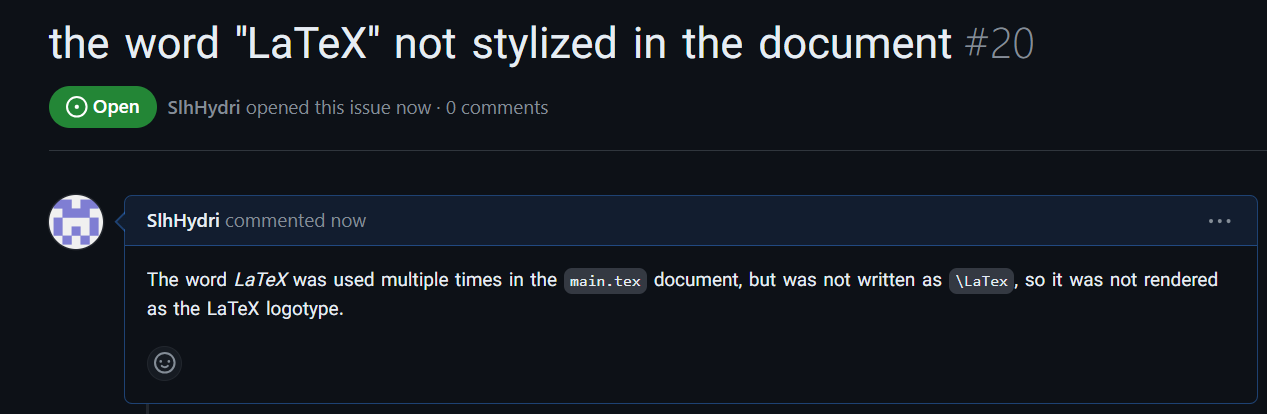
\includegraphics[width=0.9\textwidth]{image.png}
		\caption{A not-so-serious issue}
	\end{figure}
\end{document}